\section{Post-primary split, rank and budget sensitivity}
\label{sec:robustness}
\begin{table}[htbp]
\centering\small
\caption{Study stages and their evidential roles. Acquisition seeds vary order/ties unless cell-order variation is explicitly stated. Reused data/worlds do not supply independent biological replication.}
\label{tab:study}
\begin{tabular}{>{\raggedright\arraybackslash}p{.19\linewidth}>{\raggedright\arraybackslash}p{.35\linewidth}>{\raggedright\arraybackslash}p{.36\linewidth}}
\toprule
Stage & Scope & Role and timing\\
\midrule
Controlled & 14 scenarios, five worlds, five acquisition seeds; 96--192 & Known truth and failures; original settings, reused worlds\\
Development & Frangieh Control to IFN$\gamma$; 205 targets & Grid/weight selection; separate 6,428-unit exposure\\
Frozen primary & Both K562/RPE1 directions; one split, rank 4; 128--512; five seeds & Pre-scoring component comparison; fixed cell banks\\
Secondary & Prices 0/16/64; ranking, resampling, direct queries & Declared post-primary diagnostics; distinct information/cost scopes\\
PI robustness & Two new split/cell-order seeds; both directions; ranks 4/16; 128--2,048; three seeds & Post-primary sensitivity; all eight cells retained, data reused\\
\bottomrule
\end{tabular}
\end{table}

All eight additional runs completed, yielding 360 jointly closed checkpoints, 72 paid ledgers and 330,120 metric rows. Every policy/checkpoint reaches its exact budget ceiling. Figure~\ref{fig:robustness} shows all 32 extension contrasts: two query-design references and two budget grids per matrix cell. Tables~\ref{tab:robust-full} and \ref{tab:robust-original} retain absolute differences and conditional query ranges. The shorter grid reuses these new predictions at 128/256/512; it is not a new execution of the original fixed split.

On the full 128--2,048 grid, six of eight point contrasts favor worst-query and two favor the extension. Against mean-query the extension instead improves in five of eight cells. For split 20261023, forward rank four improves by $3.581\%$ versus worst-query ($\Delta=-.000301735$, conditional query range $[-.000570608,-.000051932]$) and $7.215\%$ versus mean-query. The benefit is already present on this split's shorter grid ($-3.435\%$ versus worst-query); extending the budget cannot be identified as its cause. For split 20261024, both forward ranks worsen versus worst-query. At reverse rank 16, split 20261023 changes from $-.100\%$ on the shorter grid to $+.308\%$ on the full grid. A blanket negative conclusion would conceal these changes.

The favorable full-grid aggregate is heterogeneous: only 47/131 query-averaged differences favor the extension versus worst-query, with median $+.000136211$. Deleting any one query leaves the mean negative, between $-.000331337$ and $-.000234779$. Thus the mean benefit is not a uniform query-level benefit or a single-query sign artifact. All 32 contrasts have retained deletion diagnostics, with no query excluded.

Table~\ref{tab:robust-absolute} places these contrasts beside zero and both design references. Rank-four full-grid error reductions versus zero are $10.485\%$ and $7.635\%$ forward, and $2.355\%$ and $2.098\%$ reverse. These larger gains differ from the original low-budget replay; new-grid direction/rank or prospective biological utility has not been established by these squared-error improvements.

\begin{table}[htbp]
\centering\footnotesize
\caption{Full-grid absolute error areas in units $10^{-3}$, including zero $A_0$ and the extension $A_E$, worst-query $A_W$ and mean-query $A_M$ with the same paid-validation ridge predictor. The last column compares the extension with zero. Split abbreviations match Table~\ref{tab:robust-full}. Zero is a standalone zero-recipient-cost prediction reference.}
\label{tab:robust-absolute}
\begin{tabular}{lrrrrrrr}
\toprule
Direction & Split & Rank & $A_E$ & $A_W$ & $A_M$ & $A_0$ & vs zero (\%) \\
\midrule
K562$\to$RPE1 & 23 & 4 & 8.12479 & 8.42652 & 8.75659 & 9.07645 & -10.485 \\
K562$\to$RPE1 & 23 & 16 & 8.70592 & 8.73236 & 8.71399 & 9.07645 & -4.082 \\
RPE1$\to$K562 & 23 & 4 & 5.54890 & 5.53285 & 5.60994 & 5.68274 & -2.355 \\
RPE1$\to$K562 & 23 & 16 & 5.63287 & 5.61557 & 5.58358 & 5.68274 & -0.878 \\
K562$\to$RPE1 & 24 & 4 & 7.18888 & 7.15327 & 7.35413 & 7.78312 & -7.635 \\
K562$\to$RPE1 & 24 & 16 & 7.70347 & 7.67155 & 7.63943 & 7.78312 & -1.023 \\
RPE1$\to$K562 & 24 & 4 & 5.58514 & 5.56886 & 5.63921 & 5.70480 & -2.098 \\
RPE1$\to$K562 & 24 & 16 & 5.65098 & 5.63900 & 5.64380 & 5.70480 & -0.943 \\
\bottomrule
\end{tabular}

\end{table}

\begin{figure}[htbp]
\centering
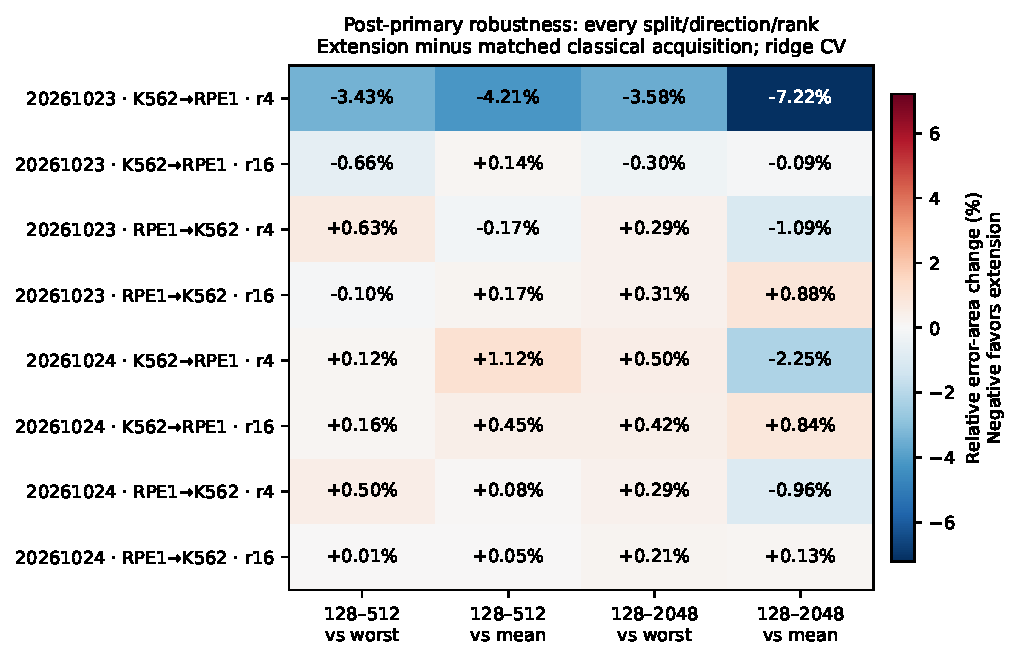
\includegraphics[width=\linewidth]{figures/robustness-matrix.pdf}
\caption{Every post-primary robustness cell. Percent changes use each reference's own error area; negative favors the fixed-RBF extension with the same paid-validation ridge predictor. The original subgrid uses 128/256/512 and the full grid adds 1,024/2,048. Colors and numbers are descriptive point estimates, not multiplicity-adjusted evidence or eight independent trials. Absolute paired differences and conditional query ranges are reported in the accompanying tables.}
\label{fig:robustness}
\end{figure}

\begin{table}[htbp]
\centering\footnotesize
\caption{All wider-grid robustness contrasts (128--2,048), in units $10^{-5}$. $\Delta_W$/$\Delta_M$ compare the extension with worst/mean query. Ranges are conditional query resampling, with three acquisition seeds averaged within query. Split 23/24 abbreviates 20261023/20261024. Negative favors the extension; no biological or multiple-comparison interpretation is assigned.}
\label{tab:robust-full}
\begin{tabular}{lrrrrrr}
\toprule
Direction & Split & Rank & $\Delta_W$ & Query range & $\Delta_M$ & Query range \\
\midrule
K562$\to$RPE1 & 23 & 4 & -30.174 & [-57.061, -5.193] & -63.181 & [-107.791, -22.524] \\
K562$\to$RPE1 & 23 & 16 & -2.644 & [-9.552, +5.503] & -0.807 & [-13.299, +11.646] \\
RPE1$\to$K562 & 23 & 4 & +1.605 & [-1.921, +6.252] & -6.104 & [-12.337, -0.916] \\
RPE1$\to$K562 & 23 & 16 & +1.730 & [+0.054, +3.295] & +4.929 & [+2.298, +7.684] \\
K562$\to$RPE1 & 24 & 4 & +3.562 & [-10.151, +17.193] & -16.525 & [-38.348, +3.963] \\
K562$\to$RPE1 & 24 & 16 & +3.192 & [-0.178, +6.982] & +6.404 & [-10.812, +24.471] \\
RPE1$\to$K562 & 24 & 4 & +1.628 & [-0.484, +4.344] & -5.407 & [-12.695, +0.485] \\
RPE1$\to$K562 & 24 & 16 & +1.198 & [+0.288, +2.279] & +0.717 & [+0.028, +1.528] \\
\bottomrule
\end{tabular}

\end{table}

Unlike rank four, rank 16 is estimated-unsupported for every query at budget 128, then fully supported from budget 256 onward for every policy and cell. This directly challenges the original already-supported regime. It still concerns estimated source coordinates, not oracle biological support. Extension/ridge selects zero in 9/60 rank-four and 10/60 rank-16 fits; at budget 128 this occurs in 8/12 fits for each rank. There are no extension null selections at 512, 1,024 or 2,048. The largest ridge penalty is selected in 9/60 and 30/60 fits, respectively. Support changes and shrinkage therefore coexist; a weak-prior acquisition variance remains distinct from actual prediction risk. Complete per-budget penalties, controls, opened identities and source-half shifts are retained.

These repeated episodes are dependent. Original--new query overlaps are 31/131 and 33/131; the two new splits share 35/131 queries. Within a direction all 50,912 source cells are shared. Across same-direction split pairs, acquisition banks overlap by 12,730--12,864 cells, query assessment by 316--363 and assessment controls by 121--131. In the opposite direction the supplied source includes all 4,448 cells used by the other task's scorer. Each task obeys its own declared information boundary, but this role reuse prevents treating the matrix as new untouched external validation. No pooling or subgroup selection converts these exploratory contrasts into a renewed primary result.

\begin{table}[htbp]
\centering\footnotesize
\caption{The same new robustness runs restricted to the 128--512 subgrid. Units, sign, split labels and conditional ranges match Table~\ref{tab:robust-full}. Three of eight point contrasts favor the extension against worst-query and two of eight against mean-query. All cells remain visible regardless of direction or sign.}
\label{tab:robust-original}
\begin{tabular}{lrrrrrr}
\toprule
Direction & Split & Rank & $\Delta_W$ & Query range & $\Delta_M$ & Query range \\
\midrule
K562$\to$RPE1 & 23 & 4 & -30.611 & [-60.093, -4.850] & -37.794 & [-69.811, -9.103] \\
K562$\to$RPE1 & 23 & 16 & -5.962 & [-10.975, -1.637] & +1.229 & [-4.039, +7.073] \\
RPE1$\to$K562 & 23 & 4 & +3.530 & [+0.439, +7.564] & -0.968 & [-2.040, -0.036] \\
RPE1$\to$K562 & 23 & 16 & -0.565 & [-1.142, -0.074] & +0.973 & [-0.204, +2.267] \\
K562$\to$RPE1 & 24 & 4 & +0.907 & [-13.166, +15.911] & +8.482 & [-11.522, +30.455] \\
K562$\to$RPE1 & 24 & 16 & +1.269 & [-0.500, +3.530] & +3.450 & [-5.814, +14.126] \\
RPE1$\to$K562 & 24 & 4 & +2.814 & [-0.282, +6.610] & +0.471 & [+0.189, +0.801] \\
RPE1$\to$K562 & 24 & 16 & +0.041 & [-0.035, +0.126] & +0.265 & [-0.103, +0.705] \\
\bottomrule
\end{tabular}

\end{table}
